% ==========================================================
%  Computer Vision — Master Summary
%  Based on summary_template.tex design philosophy.
% ==========================================================

\documentclass[11pt, oneside]{book}


% ══════════════════════════════════════════════════════════
%  PAGE GEOMETRY
% ══════════════════════════════════════════════════════════
\usepackage[
  a4paper,
  top    = 2.6cm,
  bottom = 2.1cm,
  left   = 2.5cm,
  right  = 2.5cm,
  headheight = 15pt
]{geometry}


% ══════════════════════════════════════════════════════════
%  TYPOGRAPHY
% ══════════════════════════════════════════════════════════
\usepackage[T1]{fontenc}
\usepackage[utf8]{inputenc}
\usepackage{lmodern}
\usepackage{microtype}
\usepackage{inconsolata}

\setlength{\parindent}{0pt}
\setlength{\parskip}{0.62em}


% ══════════════════════════════════════════════════════════
%  MATHEMATICS
% ══════════════════════════════════════════════════════════
\usepackage{amsmath, amssymb, amsthm, mathtools}
\usepackage{bm}
\usepackage{bbm}
\usepackage{mathrsfs}
\usepackage{nicefrac}
\usepackage{cancel}


% ══════════════════════════════════════════════════════════
%  SCIENTIFIC NOTATION
% ══════════════════════════════════════════════════════════
\usepackage{siunitx}
\sisetup{per-mode = symbol}

\usepackage[version=4]{mhchem}


% ══════════════════════════════════════════════════════════
%  FIGURES, TABLES, LISTS
% ══════════════════════════════════════════════════════════
\usepackage{graphicx}
\usepackage{subcaption}
\usepackage{booktabs}
\usepackage{array}
\usepackage{float}
\usepackage{enumitem}

\setlist[itemize]{topsep=3pt, itemsep=2pt, leftmargin=2.2em}
\setlist[enumerate]{topsep=3pt, itemsep=2pt, leftmargin=2.4em}

\usepackage{tikz}
\usetikzlibrary{positioning,arrows.meta}

\graphicspath{{figures/}}


% ══════════════════════════════════════════════════════════
%  ALGORITHMS / PSEUDOCODE
% ══════════════════════════════════════════════════════════
\usepackage[ruled, vlined, linesnumbered]{algorithm2e}
\SetAlFnt{\small}
\SetAlCapFnt{\small\bfseries}
\SetCommentSty{textit}


% ══════════════════════════════════════════════════════════
%  COLORS
% ══════════════════════════════════════════════════════════
\usepackage{xcolor}

\definecolor{accent}{HTML}{1B3A5C}

\definecolor{def@frame}{HTML}{1A5276}   \definecolor{def@bg}{HTML}{EBF5FB}
\definecolor{thm@frame}{HTML}{922B21}   \definecolor{thm@bg}{HTML}{FDEDEC}
\definecolor{ex@frame} {HTML}{1E8449}   \definecolor{ex@bg} {HTML}{EAFAF1}
\definecolor{int@frame}{HTML}{9A6A00}   \definecolor{int@bg}{HTML}{FEF9E7}
\definecolor{note@frame}{HTML}{5B2C6F}  \definecolor{note@bg}{HTML}{F5EEF8}


% ══════════════════════════════════════════════════════════
%  CODE LISTINGS
% ══════════════════════════════════════════════════════════
\usepackage{listings}
\lstset{
  basicstyle       = \ttfamily\small,
  breaklines       = true,
  numbers          = left,
  numberstyle      = \tiny\color{gray!70},
  frame            = tb,
  framerule        = 0.4pt,
  rulecolor        = \color{gray!35},
  tabsize          = 2,
  showstringspaces = false,
  keywordstyle     = \color{def@frame}\bfseries,
  commentstyle     = \color{gray!55!black}\itshape,
  stringstyle      = \color{ex@frame!90!black},
  backgroundcolor  = \color{gray!5},
  xleftmargin      = 2em,
  xrightmargin     = 0.4em,
  aboveskip        = 0.8em,
  belowskip        = 0.5em
}


% ══════════════════════════════════════════════════════════
%  CUSTOM BOXES  (tcolorbox)
% ══════════════════════════════════════════════════════════
\usepackage[most]{tcolorbox}

\tcbset{
  enhanced,
  breakable,
  arc             = 2.5mm,
  boxrule         = 0.5pt,
  left            = 4.5mm,
  right           = 4mm,
  top             = 2.5mm,
  bottom          = 2.5mm,
  fonttitle       = \bfseries\small,
  sharp corners   = west,
  parbox          = false
}

\newtcolorbox{defbox}[1][]{
  title  = {Definition},
  colback = def@bg, colframe = def@frame,
  borderline west = {3.5pt}{0pt}{def@frame},
  #1
}

\newtcolorbox{thmbox}[1][]{
  title  = {Theorem / Key Formula},
  colback = thm@bg, colframe = thm@frame,
  borderline west = {3.5pt}{0pt}{thm@frame},
  #1
}

\newtcolorbox{exbox}[1][]{
  title  = {Example},
  colback = ex@bg, colframe = ex@frame,
  borderline west = {3.5pt}{0pt}{ex@frame},
  #1
}

\newtcolorbox{intbox}[1][]{
  title  = {Intuition \& Mental Model},
  colback = int@bg, colframe = int@frame,
  borderline west = {3.5pt}{0pt}{int@frame},
  #1
}

\newtcolorbox{notebox}[1][]{
  title  = {Note},
  colback = note@bg, colframe = note@frame,
  borderline west = {3.5pt}{0pt}{note@frame},
  #1
}


% ══════════════════════════════════════════════════════════
%  TABLE OF CONTENTS  (tocloft)
% ══════════════════════════════════════════════════════════
\usepackage[titles]{tocloft}

\renewcommand{\cftchapfont}     {\bfseries\color{accent}}
\renewcommand{\cftchappagefont} {\bfseries\color{accent}}
\renewcommand{\cftchapleader}   {\bfseries\color{accent!40}\cftdotfill{\cftdotsep}}
\setlength{\cftbeforechapskip} {7pt}

\renewcommand{\cftsecfont}      {\small}
\renewcommand{\cftsecpagefont}  {\small}
\setlength{\cftsecindent}      {1.8em}
\setlength{\cftbeforesecskip}  {1.5pt}

\renewcommand{\cftsubsecfont}      {\small\color{gray!65!black}}
\renewcommand{\cftsubsecpagefont}  {\small\color{gray!65!black}}
\setlength{\cftsubsecindent}      {3.4em}
\setlength{\cftbeforesubsecskip}  {0.5pt}


% ══════════════════════════════════════════════════════════
%  CHAPTER & SECTION HEADINGS  (titlesec)
% ══════════════════════════════════════════════════════════
\usepackage{titlesec}

\titleformat{\chapter}[display]
  {\normalfont\bfseries\color{accent}\huge}
  {\hfill\fontsize{68}{68}\selectfont\color{accent!13}\thechapter}
  {-10pt}
  {}
  [{\vspace{4pt}%
    {\color{accent}\rule{\linewidth}{1.6pt}}\\[-2pt]%
    {\color{accent!35}\rule{\linewidth}{0.5pt}}}]
\titlespacing*{\chapter}{0pt}{-28pt}{22pt}

\titleformat{\section}
  {\normalfont\large\bfseries\color{accent}}
  {\thesection}
  {0.8em}
  {}
  [{\vspace{1pt}\color{accent!45}\titlerule[0.45pt]}]
\titlespacing*{\section}{0pt}{3.8ex plus 1ex minus .2ex}{2.2ex plus .2ex}

\titleformat{\subsection}
  {\normalfont\normalsize\bfseries\color{accent!80!black}}
  {\thesubsection}
  {0.7em}
  {}
\titlespacing*{\subsection}{0pt}{2.6ex plus 1ex minus .2ex}{1.4ex plus .2ex}

\titleformat{\paragraph}[runin]
  {\normalfont\small\bfseries}
  {}
  {0em}
  {}[.\enspace]
\titlespacing{\paragraph}{0pt}{1.2ex plus .5ex minus .2ex}{0.5em}


% ══════════════════════════════════════════════════════════
%  HEADER & FOOTER
% ══════════════════════════════════════════════════════════
\usepackage{fancyhdr}
\pagestyle{fancy}
\fancyhf{}
\fancyhead[L]{\small\color{gray!70}\nouppercase{\leftmark}}
\fancyhead[R]{\small\color{gray!70}\thepage}
\renewcommand{\headrulewidth}{0.4pt}

\fancypagestyle{plain}{%
  \fancyhf{}
  \fancyfoot[C]{\small\color{gray!70}\thepage}
  \renewcommand{\headrulewidth}{0pt}%
}


% ══════════════════════════════════════════════════════════
%  LINKS & REFERENCES
% ══════════════════════════════════════════════════════════
\usepackage[hidelinks]{hyperref}
\usepackage[nameinlink, capitalize]{cleveref}


% ══════════════════════════════════════════════════════════
%  DOCUMENT METADATA
% ══════════════════════════════════════════════════════════
\newcommand{\coursetitle}{Computer Vision}
\newcommand{\documenttype}{Master Summary}
\newcommand{\authorname}{Stefan Eder}
\newcommand{\basedon}{Based on Lecture \emph{Computer Vision} SS26}


% ══════════════════════════════════════════════════════════
%  MATHEMATICAL MACROS
% ══════════════════════════════════════════════════════════

% ── Number Sets & Spaces ──────────────────────────────────
\newcommand{\R}{\mathbb{R}}
\newcommand{\N}{\mathbb{N}}
\newcommand{\Z}{\mathbb{Z}}
\newcommand{\C}{\mathbb{C}}
\newcommand{\Q}{\mathbb{Q}}

% ── Probability & Statistics ──────────────────────────────
\newcommand{\E}{\mathbb{E}}
\newcommand{\Prob}{\mathbb{P}}
\newcommand{\Var}{\mathrm{Var}}
\newcommand{\Cov}{\mathrm{Cov}}
\newcommand{\Corr}{\mathrm{Corr}}
\newcommand{\iid}{\overset{\mathrm{iid}}{\sim}}
\newcommand{\ind}{\mathbbm{1}}

% ── Information Theory ────────────────────────────────────
\newcommand{\KL}[2]{D_{\mathrm{KL}}\!\left(#1 \,\|\, #2\right)}
\newcommand{\Ent}{\mathrm{H}}
\newcommand{\MI}{\mathrm{I}}

% ── Calculus & Optimization ───────────────────────────────
\newcommand{\argmax}{\operatorname*{arg\,max}}
\newcommand{\argmin}{\operatorname*{arg\,min}}
\newcommand{\grad}{\nabla}
\newcommand{\hess}{\nabla^2}
\newcommand{\lapl}{\Delta}
\newcommand{\dd}{\,\mathrm{d}}
\newcommand{\pd}[2]{\frac{\partial #1}{\partial #2}}
\newcommand{\pdd}[2]{\frac{\partial^2 #1}{\partial #2^2}}

% ── Norms, Abs, Inner Products ────────────────────────────
\newcommand{\norm}[1]{\left\lVert #1 \right\rVert}
\newcommand{\normsq}[1]{\left\lVert #1 \right\rVert^2}
\newcommand{\abs}[1]{\left\lvert #1 \right\rvert}
\newcommand{\inner}[2]{\left\langle #1,\, #2 \right\rangle}

% ── Linear Algebra ────────────────────────────────────────
\newcommand{\T}{^{\mathsf{T}}}
\newcommand{\inv}{^{-1}}
\newcommand{\pinv}{^{\dagger}}
\newcommand{\tr}{\operatorname{tr}}
\newcommand{\rank}{\operatorname{rank}}
\newcommand{\diag}{\operatorname{diag}}
\newcommand{\spanop}{\operatorname{span}}
\newcommand{\eye}{\mathbf{I}}
\newcommand{\zeros}{\mathbf{0}}
\newcommand{\ones}{\mathbf{1}}

% ── ML / AI Core Notation ────────────────────────────────
\newcommand{\loss}{\mathcal{L}}
\newcommand{\reg}{\mathcal{R}}
\newcommand{\dataset}{\mathcal{D}}
\newcommand{\params}{\boldsymbol{\theta}}
\newcommand{\weights}{\mathbf{w}}
\newcommand{\xvec}{\mathbf{x}}
\newcommand{\yvec}{\mathbf{y}}
\newcommand{\zvec}{\mathbf{z}}
\newcommand{\hvec}{\mathbf{h}}
\newcommand{\feature}{\boldsymbol{\phi}}

% Activation functions
\DeclareMathOperator{\softmax}{softmax}
\DeclareMathOperator{\relu}{ReLU}
\DeclareMathOperator{\sign}{sign}

% ── Complexity ────────────────────────────────────────────
\newcommand{\bigO}[1]{\mathcal{O}\!\left(#1\right)}
\newcommand{\bigOm}[1]{\Omega\!\left(#1\right)}
\newcommand{\bigTh}[1]{\Theta\!\left(#1\right)}

% ── Common Distributions ──────────────────────────────────
\newcommand{\Normal}{\mathcal{N}}
\newcommand{\Uniform}{\mathcal{U}}
\newcommand{\Bernoulli}{\mathrm{Ber}}
\newcommand{\Categorical}{\mathrm{Cat}}
\newcommand{\Dirichlet}{\mathrm{Dir}}
\newcommand{\Binomial}{\mathrm{Bin}}

% ── Miscellaneous ─────────────────────────────────────────
\newcommand{\given}{\,\vert\,}
\newcommand{\st}{\;\text{s.t.}\;}
\newcommand{\eqdef}{\coloneqq}
\newcommand{\eqq}{\overset{?}{=}}

% ── Computer Vision ───────────────────────────────────────
\newcommand{\vct}[1]{\bm{#1}}           % vector (bold italic)
\newcommand{\mat}[1]{\mathbf{#1}}       % matrix (bold upright)

% ── Convenience ───────────────────────────────────────────
\newcommand{\TODO}[1]{\textcolor{gray}{\emph{TODO: #1}}}


% ==========================================================
%  BEGIN DOCUMENT
% ==========================================================
\begin{document}

\frontmatter


% ──────────────────────────────────────────────────────────
%  TITLE PAGE
% ──────────────────────────────────────────────────────────
\thispagestyle{empty}
\vspace*{1.8cm}

\begin{center}
  {\color{accent}\rule{\linewidth}{1.8pt}}
  \vspace{0.65cm}

  {\fontsize{28}{34}\selectfont\bfseries\color{accent}\coursetitle\par}
  \vspace{0.25cm}
  {\large\color{gray!80!black}\documenttype\par}

  \vspace{0.55cm}
  {\color{accent!35}\rule{\linewidth}{0.5pt}}
  \vspace{0.55cm}

  {\large\authorname\par}
  \vspace{0.2cm}
  {\small\color{gray!70}\basedon\par}
\end{center}

\vspace{1.6cm}

\begin{center}
\begin{minipage}{0.84\textwidth}
  \small\color{gray!80!black}
  This document is a compact summary of the course.
  It aims to cover all relevant concepts and results, but long derivations,
  detailed proofs, and worked examples are often condensed or omitted in
  favour of clarity and conciseness.
  Use it as a study aid alongside the lecture notes and slides, not as a
  replacement for them.

  \medskip
  If you spot an error or a gap, please open an issue or pull request at
  \textbf{github.com/stevetgit} --- corrections are always welcome.

  \medskip
  \color{gray!60!black}
  Good study materials should be shared, not gatekept.
  If this helped you, take it as a reason to help the next colleague you see struggling with something.
\end{minipage}
\end{center}

\vfill
{\centering\small\color{gray!65} \today\par}
\clearpage


% ──────────────────────────────────────────────────────────
%  TABLE OF CONTENTS
% ──────────────────────────────────────────────────────────
\setcounter{tocdepth}{2}

\begingroup
  \let\cleardoublepage\relax
  \let\clearpage\relax
  \tableofcontents
\endgroup

\mainmatter


% ==========================================================
%  CHAPTER 1 — INTRODUCTION
% ==========================================================
\chapter{Introduction}

Computer Vision studies how to \emph{extract information from visual observations}
(images and videos) in order to \emph{understand} a scene and act on it.
Typical outputs include labels, locations, motion estimates, geometry (depth and 3D structure),
and pixel-level interpretations.
The field sits at the intersection of optics, signal processing, and machine learning.

\begin{defbox}[title={Computer Vision}]
\textbf{Computer Vision (CV)} is the discipline of designing algorithms and systems that
automatically interpret visual data. Outputs include class labels, object locations, 2D motion fields,
dense depth maps, and full 3D reconstructions.
\end{defbox}

The pipeline from scene to inference can be summarized as:

\begin{center}
\begin{tikzpicture}[
  node distance=12mm,
  >=Latex,
  every node/.style={draw, rounded corners, inner sep=4pt, font=\small}
]
  \node (world) {3D world + illumination};
  \node[right=12mm of world] (sensor) {optics \& sensor};
  \node[right=12mm of sensor] (img) {image / video};
  \node[right=12mm of img] (repr) {representation};
  \node[right=12mm of repr] (inf) {inference};

  \draw[->] (world) -- (sensor);
  \draw[->] (sensor) -- (img);
  \draw[->] (img) -- (repr);
  \draw[->] (repr) -- (inf);

  \node[below=4mm of repr, draw=none, align=center, text width=40mm]
    {features / descriptors\\or learned embeddings};
  \node[below=4mm of inf, draw=none, align=center, text width=36mm]
    {task output\\(label, motion, depth, \dots)};
\end{tikzpicture}
\end{center}

\begin{intbox}
Vision is an \textbf{inverse problem}: many different 3D scenes can produce very similar (or identical) 2D images.
To do well, a system needs \textbf{assumptions} (priors) about the world.
\end{intbox}

Several fundamental difficulties make CV challenging:
\begin{itemize}
  \item \textbf{Information loss:} projection from 3D to 2D removes depth; occlusions hide parts of the scene.
  \item \textbf{Appearance variation:} illumination, viewpoint, shadows, specularities, and sensor noise change pixel values.
  \item \textbf{Local ambiguity:} textureless regions and repeated patterns make matching and motion estimation ill-posed (aperture-style issues).
  \item \textbf{Scale and context:} what something \emph{is} may depend on global context rather than local pixels.
\end{itemize}

\section{Classical CV Task Landscape}

The lecture highlights three core task families that recur throughout the course:
\begin{itemize}
  \item \textbf{Classification / recognition:} what is in the image? (object, category, and scene labels).
  \item \textbf{Motion estimation and tracking:} how do pixels and objects move over time? (e.g., optical flow, tracking).
  \item \textbf{Scene reconstruction:} recover geometry (depth and 3D structure) from one or multiple images.
\end{itemize}

Many other tasks --- segmentation, detection, pose estimation, SLAM --- can be seen as combinations
or refinements of the above and will appear in later chapters.


% ==========================================================
%  CHAPTER 2 — CAPTURING DIGITAL IMAGES
% ==========================================================
\chapter{Capturing Digital Images}

Every CV pipeline starts with image formation: how does light from a 3D scene become a discrete array of numbers?
This chapter traces the path from physical optics through camera geometry to calibration and active sensors.

\section{Image Formation Models}

\subsection{Pinhole Camera and Perspective Projection}

The simplest camera model places a single aperture (the pinhole) between the scene and the image plane.
All light from a scene point must pass through the pinhole, so each scene point maps to exactly one image point.

\begin{defbox}[title={Pinhole Camera}]
A \textbf{pinhole camera} maps a 3D point $\vct{P}=(X,Y,Z)\T$ in camera coordinates to an image point
$\vct{p}=(x,y)\T$ by intersecting the ray from $\vct{P}$ through a single aperture with the image plane.
\end{defbox}

\begin{thmbox}[title={Perspective Projection}]
For a camera coordinate system with image plane at distance $f$:
\[
x = \frac{fX}{Z},\qquad y = \frac{fY}{Z}.
\]
\end{thmbox}

There is an inherent trade-off in pinhole size: a smaller pinhole yields a sharper image (less geometric blur)
but lets in less light. A larger pinhole is brighter but blurrier, because rays from one scene point spread
over an area on the image plane.
In practice, a \emph{virtual image plane in front of the pinhole} is often used to avoid the ``flipped image''
mental picture; the mathematics stays the same.

\subsection{Projection Models: Perspective, Orthographic, and Weak Perspective}

Real cameras and CV algorithms use several approximations of perspective projection depending on
the depth variation in the scene.

\begin{defbox}[title={Projection Models}]
\textbf{Perspective projection} scales by inverse depth $1/Z$ (farther objects appear smaller). \\
\textbf{Orthographic/Parallel projection} ignores depth scaling (reasonable if depth variation is small). \\
\textbf{Weak perspective (scaled orthographic)} approximates all depths in a region by a constant reference depth
$Z_0$ (e.g.\ the mean object depth), so perspective becomes a \emph{constant-scale} projection.
\end{defbox}

\begin{thmbox}[title={Projection Equations}]
Let $(X,Y,Z)$ be camera coordinates and $(x,y)$ normalized image coordinates.

\begin{align*}
\textbf{Perspective:}\quad
& x = \frac{X}{Z}, \qquad y = \frac{Y}{Z}. \\[2pt]
\textbf{Weak perspective:}\quad
& \text{assume } Z = Z_0 + \Delta Z \text{ with } |\Delta Z|\ll Z_0 \\
& \Rightarrow\; x \approx \frac{X}{Z_0}, \qquad y \approx \frac{Y}{Z_0}
\quad \text{(constant scale within the region)} \\
\textbf{Orthographic/Parallel:}\quad
& x = X, \qquad y = Y
\quad \text{(optionally with a constant scale factor } s\text{).}
\end{align*}
\end{thmbox}

In perspective projection, 3D parallel lines can meet at a \emph{vanishing point} in the image,
and the \emph{horizon line} is the set of vanishing points for directions parallel to the ground plane.
In (weak) orthographic projection, parallel lines remain parallel --- there are no vanishing points.

\begin{center}
  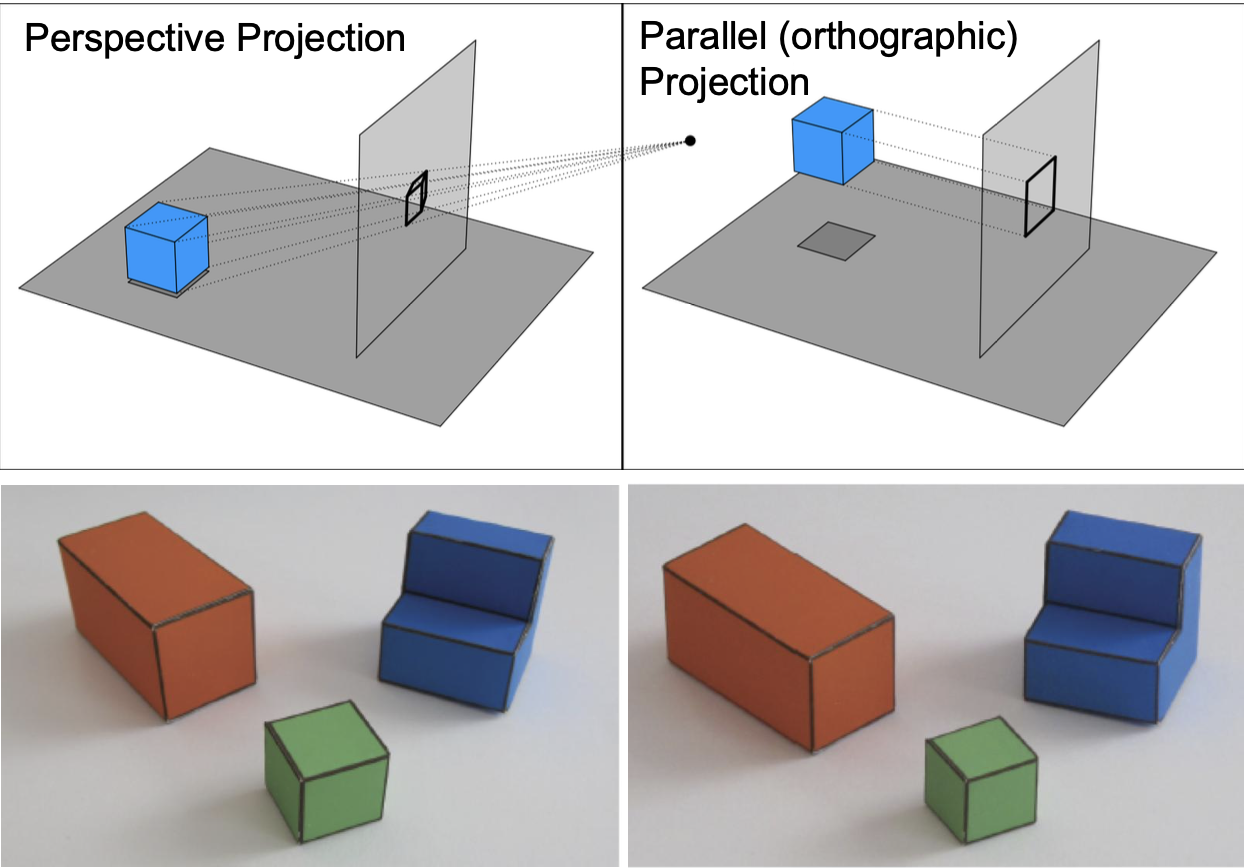
\includegraphics[width=0.7\linewidth]{projection.png}
\end{center}

\subsection{Thin Lens Model: Focal Length, Focus, and Aperture}

Real cameras use lenses to collect more light than a pinhole while keeping points approximately focused.
Despite using a thin lens, the mapping from 3D to 2D is still well-approximated by the linear projective
(pinhole) model; more complex or thick lenses primarily require non-linear distortion models in practice.

\begin{defbox}[title={Focal Length}]
The \textbf{focal length $f$} is the distance from the (thin) lens center to the focal point where parallel
incoming rays (from infinity) converge.
\end{defbox}

\begin{defbox}[title={Aperture}]
An adjustable opening controlling the \emph{effective diameter} of the lens (how many rays are admitted).
\end{defbox}

Although a lens is used for light collection and focusing, the \emph{geometric mapping} from 3D to 2D is
still well approximated by the same perspective projection equations as the pinhole model --- the lens
mainly improves brightness by capturing rays from a finite solid angle.

\subsection{Depth of Field and f-Number}

\begin{defbox}[title={Depth of Field}]
The \textbf{depth of field (DoF)} is the range of depths that appear acceptably sharp in the image.
\end{defbox}

\begin{thmbox}[title={f-Number}]
The \textbf{f-number} $N$ is a dimensionless ratio
\[
N=\frac{f}{D}
\qquad\Longleftrightarrow\qquad
D=\frac{f}{N},
\]
where $f$ is the focal length and $D$ is the effective aperture diameter (entrance pupil).
\end{thmbox}

\begin{itemize}
  \item \textbf{Larger $N$} (smaller aperture): \emph{less light} but \emph{larger DoF} (more of the scene appears sharp).
  \item \textbf{Smaller $N$} (larger aperture): \emph{more light} but \emph{smaller DoF} (stronger background blur).
\end{itemize}

Collected light is proportional to the aperture area, so
\[
\text{light} \propto D^2 \propto \frac{1}{N^2}.
\]
Changing the f-number by one full ``stop'' changes the light by roughly a factor of 2.

\begin{exbox}[title={f-Number Calculation}]
If $f=\SI{80}{mm}$ and $N=4$, then $D=f/N=\SI{20}{mm}$.
\end{exbox}

\begin{defbox}[title={Geometric Lens Distortion}]
\textbf{Geometric lens distortion} warps image geometry. Most important in CV: \textbf{radial distortion}
(barrel vs.\ pincushion), especially for wide FoV lenses. Most consumer cameras need calibration before use in CV.
\end{defbox}

\section{Digital Sensors and the Imaging Pipeline}

\subsection{Sampling and Quantization}

\begin{defbox}[title={Digital Image}]
A digital image is a discrete 2D function:
\[
I:\{1,\dots,W\}\times\{1,\dots,H\}\to \{0,\dots,2^b-1\},
\]
where $b$ is the \textbf{bit depth} (e.g., $b=8$ for 256 intensity levels).
\end{defbox}

\begin{itemize}
  \item \textbf{Sampling} (finite pixel spacing) limits spatial resolution.
  \item \textbf{Aliasing} occurs when scene detail exceeds the sensor sampling rate (high frequencies fold into low ones).
  \item \textbf{Quantization} maps continuous irradiance to discrete intensity values; larger $b$ gives finer intensity steps.
\end{itemize}

Anti-aliasing can be helped by optical blur (lens and sensor) or explicit low-pass filtering before downsampling.

\subsection{Noise Sources and SNR}

\begin{defbox}[title={Noise and SNR}]
\textbf{Noise} is random variation in the measured pixel value under identical conditions.
The \textbf{signal-to-noise ratio (SNR)} is often more informative than absolute noise.
\end{defbox}

\begin{itemize}
  \item \textbf{Shot noise:} photon counting statistics (Poisson distributed). For large photon counts, Poisson is well-approximated by a Gaussian.
  \item \textbf{Read noise:} sensor and electronics noise (approximately signal-independent).
  \item \textbf{Exposure trade-off:} more exposure (time or aperture) increases signal and usually improves SNR, but may cause motion blur or saturation.
\end{itemize}

Averaging multiple independent frames reduces noise variance (roughly $\propto 1/n$) and improves SNR.

Many consumer cameras apply a \textbf{non-linear response} (gamma-like) to mimic human perception.
For CV it is often beneficial to \textbf{linearize} intensities before photometric computations.
If starting from raw Bayer/CFA data, a common CV order is: \textbf{linearize raw CFA samples first, then demosaic}
(so interpolation happens in a linear domain).

\subsection{Color Filter Arrays and Demosaicing}

\begin{defbox}[title={Color Filter Array}]
Most sensors measure only \textbf{one} color per pixel using a \textbf{Color Filter Array (CFA)}.
The most common CFA is the \textbf{Bayer pattern} with twice as many green samples as red or blue:
\textbf{50\% green, 25\% red, 25\% blue}.
\end{defbox}

\textbf{Demosaicing} (debayering) interpolates the missing channels from neighbors to obtain a full RGB image.
More green samples reflect that perceived luminance is strongly influenced by green wavelengths; it also helps spatial detail.

\section{Color Imaging}

Grayscale is often sufficient for geometry and structure (edges, corners, motion) and can simplify modeling.
RGB is useful when appearance cues matter (recognition, segmentation, materials).

\textbf{White balance / color constancy} compensates for the illuminant so that neutral objects appear neutral
and colors are comparable across lighting conditions.

\section{Camera Geometry and the Camera Matrix}

\subsection{Coordinate Systems and Homogeneous Coordinates}

We distinguish three coordinate systems:
\begin{itemize}
  \item \textbf{World coordinates} $\vct{P}_W=(X_W,Y_W,Z_W)\T$: fixed scene coordinate system.
  \item \textbf{Camera coordinates} $\vct{P}_C=(X_C,Y_C,Z_C)\T$: origin at the camera center, $Z_C$ points forward.
  \item \textbf{Image / pixel coordinates} $(u,v)$: discrete pixel grid on the sensor.
\end{itemize}

\begin{defbox}[title={Homogeneous Coordinates}]
We write points with an extra coordinate so that projections become linear.
\begin{itemize}
  \item 2D point $(x,y)$ becomes $\tilde{\vct{p}}=(x,y,1)\T$ (also $(\lambda x,\lambda y,\lambda)\T$ for any $\lambda\neq 0$).
  \item 3D point $(X,Y,Z)$ becomes $\tilde{\vct{P}}=(X,Y,Z,1)\T$ (defined only up to scale).
\end{itemize}
\end{defbox}

\subsection{Perspective Division and Extrinsics}

\begin{thmbox}[title={Perspective Division}]
If $\tilde{\vct{p}}=(x',y',w')\T$ is a homogeneous image point, the Euclidean point is
\[
(x,y)=\left(\frac{x'}{w'},\frac{y'}{w'}\right).
\]
\end{thmbox}

The \textbf{extrinsics} tell us where the camera is and how it is oriented relative to the world.
$\mat{R}$ is a 3D rotation matrix ($\mat{R}^\top \mat{R}=\eye$, $\det(\mat{R})=1$, i.e.\ $SO(3)$),
and $\vct{C}\in\R^3$ is the \textbf{camera center} in world coordinates.

\begin{thmbox}[title={World to Camera Transform}]
To express a world point in the camera coordinate system:
\[
\vct{P}_C = \mat{R}\bigl(\vct{P}_W - \vct{C}\bigr) = \mat{R}\vct{P}_W + \vct{t},
\qquad
\vct{t} = -\mat{R}\vct{C}.
\]
\end{thmbox}

\subsection{Projection Matrix and Intrinsics}

\begin{thmbox}[title={Pinhole Camera Model}]
\[
\tilde{\vct{p}} \sim \mat{P}\,\tilde{\vct{P}}_W,
\qquad
\mat{P} = \mat{K}\,[\mat{R}\mid \vct{t}].
\]
\end{thmbox}

\begin{defbox}[title={Intrinsic Matrix}]
The \textbf{intrinsics} map from normalized camera coordinates to pixel coordinates.
A common intrinsic matrix form:
\[
\mat{K}=
\begin{pmatrix}
f_x & s   & c_x\\
0   & f_y & c_y\\
0   & 0   & 1
\end{pmatrix},
\]
where $(c_x,c_y)$ is the principal point, $s$ is skew (often $\approx 0$), and $f_x,f_y$ are focal lengths in pixel units.
\end{defbox}

In many calibration contexts, \textbf{intrinsics} include $(\mat{K},\text{distortion coeffs})$, i.e., lens distortion parameters
(radial and tangential) are grouped with intrinsics.

\section{Distortion and Calibration}

\subsection{Radial Distortion Model}

\begin{defbox}[title={Radial Distortion}]
The ideal pinhole model assumes rays travel perfectly straight. Real lenses bend light non-linearly near the edges,
causing \textbf{radial distortion}.
\end{defbox}

\begin{thmbox}[title={Radial Distortion Equations}]
Work in \textbf{normalized} image coordinates $(x,y)$ (after dividing by depth and removing $\mat{K}$).
Let $r^2 = x^2 + y^2$. The distortion scale factor is:
\[
s(r)= 1 + k_1 r^2 + k_2 r^4 + k_3 r^6
\]
Distorted coordinates:
\[
x_d = x\,s(r),\;\; y_d = y\,s(r).
\]
\end{thmbox}

\begin{itemize}
  \item \textbf{Barrel distortion ($k_1 < 0$):} outer points are pulled \emph{inwards}; straight lines bow outward (typical for wide-angle/fisheye lenses).
  \item \textbf{Pincushion distortion ($k_1 > 0$):} outer points are pushed \emph{outwards}; straight lines bend inward (typical for telephoto lenses).
\end{itemize}

\subsection{Checkerboard Calibration}

\begin{defbox}[title={Camera Calibration}]
Estimate intrinsics $\mat{K}$, distortion parameters, and (for each calibration image) extrinsics $(\mat{R},\vct{t})$
by observing a known pattern (e.g., checkerboard).
\end{defbox}

\begin{thmbox}[title={Reprojection Error Minimization}]
For every known 3D corner $\vct{P}_i$ on the checkerboard, project it into the image using current parameter estimates,
compare to the detected pixel $\vct{p}_i$, and minimize:
\[
\min_{\mat{K},\,\text{dist},\,\{\mat{R}_j,\vct{t}_j\}}
\sum_{j}\sum_{i}\norm{\vct{p}_{i,j} - \pi(\mat{K},\text{dist},\mat{R}_j,\vct{t}_j;\vct{P}_i)}^2.
\]
\end{thmbox}

Calibration quality is often judged by the final RMS reprojection error (smaller is better),
interpreted together with image resolution and corner detection accuracy.
Accurate $\mat{K}$ and distortion correction are prerequisites for multi-view geometry:
known relative poses $(\mat{R},\vct{t})$ allow mapping rays from different cameras into one common 3D frame.

Learning-based calibration from ``in-the-wild'' images uses: pixel-wise undistortion mappings (e.g., U-Net predicting
a dense warp), geometric cues from vanishing points/lines, or direct CNN regression of intrinsics and distortion parameters.

\section{Active Depth Sensors and Event Cameras}

\subsection{Time-of-Flight and LiDAR}

Active sensors emit structured light or laser pulses and measure the return time.
\textbf{ToF distance:} $d = \frac{c\,t}{2}$ (round-trip time $t$, speed of light $c$).
\textbf{LiDAR} is a ToF system where a laser is emitted and the return time is measured (often with scanning).

\subsection{Event Cameras (DVS)}

Standard cameras capture full frames at a fixed rate (e.g., 30 FPS), recording redundant static background
and suffering from motion blur on fast objects.
\textbf{Event cameras (DVS)} work like the human optic nerve: each pixel operates independently and only fires
an event when its brightness changes, yielding an asynchronous stream of events $(x,y,t,\text{polarity})$.
Advantages: microsecond temporal resolution, extremely low latency, no standard motion blur, and low bandwidth for static scenes.


% ==========================================================
%  CHAPTER 3 — DIGITAL IMAGE PROCESSING
% ==========================================================
\chapter{Digital Image Processing}

Digital image processing transforms pixel arrays to extract structure, remove noise, enhance features,
or prepare data for downstream analysis. The fundamental tool is the linear filter applied via convolution.

\section{Images as Discrete Signals}

\subsection{Neighborhoods and Boundary Handling}

\begin{defbox}[title={Discrete Image Signal}]
A grayscale image is a discrete 2D signal $I[n,m]$ on a pixel grid. Many operations use a local
\textbf{neighborhood} (e.g., $3\times 3$, $5\times 5$) around each pixel to compute an output.
\end{defbox}

Typical boundary handling when the neighborhood extends outside the image:
\begin{itemize}
  \item \textbf{Zero padding:} assume missing pixels are 0 (simple; can darken borders).
  \item \textbf{Replicate:} repeat boundary pixel values (often good for smoothing).
  \item \textbf{Reflect:} mirror the image at the boundary (often good for derivatives).
  \item \textbf{Circular / wrap:} treat image as periodic (matches FFT-based convolution).
\end{itemize}

Border handling changes results near image edges. For FFT-based filtering, padding the image
avoids circular wrap-around artefacts.

\subsection{Correlation vs.\ Convolution}

\begin{defbox}[title={Correlation and Convolution}]
\textbf{Correlation} applies a kernel $h$ without flipping it:
\[
(y = x \star h)\quad\Rightarrow\quad
y[m,n] = \sum_{k,l} x[m+k,n+l]\;h[k,l].
\]
\textbf{Convolution} flips the kernel in both directions:
\[
(y = x * h)\quad\Rightarrow\quad
y[m,n] = \sum_{k,l} x[m+k,n+l]\;h[-k,-l].
\]
\end{defbox}

Many CV libraries implement ``convolution'' routines that actually compute correlation
(because the kernel is learned or defined accordingly). Always check the convention.

Convolution is the prototypical \textbf{linear shift-invariant (LSI)} operation: linear combinations of inputs
map to the same linear combination of outputs, and shifting the input shifts the output.
Convolution is also \textbf{commutative, associative, and distributive}.

\section{Spatial Filtering}

\subsection{Smoothing Filters}

\begin{defbox}[title={Low-Pass Filters}]
A \textbf{low-pass filter} removes high-frequency components (fine details/noise), producing a smoother image.
The \textbf{box filter} replaces each pixel by the average of its neighborhood.
The \textbf{Gaussian filter} weights central pixels higher, forming a bell curve.
Key facts: convolution of Gaussians is Gaussian; the Fourier transform of a Gaussian is Gaussian; Gaussians are \textbf{separable}.
\end{defbox}

\subsection{Derivatives and Edges}

\begin{thmbox}[title={Image Gradient (Edge Detection)}]
Edges are strong intensity changes. Compute the gradient vector for each pixel:
\begin{enumerate}
  \item \textbf{Horizontal change ($I_x$):} convolve with Sobel $K_x$ $\left(\begin{smallmatrix}-1&0&1\\-2&0&2\\-1&0&1\end{smallmatrix}\right)$.
  \item \textbf{Vertical change ($I_y$):} convolve with $K_y=K_x^{\T}$.
  \item \textbf{Edge Strength (Magnitude):} $\norm{\nabla I} = \sqrt{I_x^2 + I_y^2}$.
  \item \textbf{Edge Direction (Orientation):} $\theta = \operatorname{atan2}(I_y, I_x)$.
\end{enumerate}
\end{thmbox}

Derivatives amplify noise. Always smooth the image first (e.g., with a Gaussian filter) before computing gradients.

\subsection{Second Derivatives and Unsharp Masking}

\begin{defbox}[title={Laplacian}]
The \textbf{Laplacian} ($\Delta I = I_{xx} + I_{yy}$) measures how much a pixel differs from the average of its
immediate neighbors. It highlights rapid changes and acts as a \textbf{high-pass filter}.
\end{defbox}

\begin{thmbox}[title={Unsharp Masking}]
\begin{enumerate}
  \item \textbf{Blur:} smooth the original image to get $I_{\text{blur}}$.
  \item \textbf{Extract Details:} $I_{\text{details}} = I - I_{\text{blur}}$.
  \item \textbf{Sharpen:} $I_{\text{sharp}} = I + \alpha\,I_{\text{details}}$.
\end{enumerate}
\end{thmbox}

Any kernel with a \textbf{large positive center} and \textbf{negative neighbors} (approximating Impulse $-$ Gaussian)
is a sharpening filter. The discrete Laplacian kernel (e.g., center 4, neighbors $-1$) performs this detail extraction in one step.

\section{Frequency Domain}

\subsection{Fourier Transform}

\begin{defbox}[title={Fourier Decomposition}]
The Fourier transform decomposes an image into a sum of 2D sine/cosine waves.
\begin{itemize}
  \item \textbf{Center (Low frequencies):} smooth gradients, global illumination, basic shapes.
  \item \textbf{Edges (High frequencies):} fine details, sharp edges, noise.
\end{itemize}
\end{defbox}

The transform produces complex numbers with two meaningful parts:
(1) \textbf{Magnitude} --- how strong is a specific frequency (the ``spectrum'');
(2) \textbf{Phase} --- where are the structures located. Phase is far more important for preserving
spatial structure and intelligibility than magnitude.

An image with \textbf{more spatial detail and sharp edges} will have a spectrum with \textbf{energy spread further out from the center} (stronger high-frequency magnitude).

\begin{thmbox}[title={Convolution Theorem}]
\[
f = g*h\ \Longleftrightarrow\ F = G\cdot H,
\]
i.e., convolution in the spatial domain corresponds to pointwise multiplication in the Fourier domain.
For large kernels, FFT-based filtering can be faster: pad image and kernel, take FFTs, multiply spectra, then inverse FFT.
\end{thmbox}

\subsection{Sampling and Aliasing}

\begin{defbox}[title={Aliasing}]
\textbf{Aliasing} occurs when sampling is too coarse: high frequencies ``fold'' into low frequencies.
To downsample safely, first low-pass filter (anti-alias filter), then subsample.
\end{defbox}

\section{Multi-Scale Representations}

\subsection{Gaussian and Laplacian Pyramids}

\begin{thmbox}[title={Gaussian Pyramid}]
To build the next smaller level of the pyramid:
\begin{enumerate}
  \item \textbf{Smooth:} apply a Gaussian filter to the current image (prevents aliasing).
  \item \textbf{Downsample:} discard every second row and column.
\end{enumerate}
Result: a set of increasingly small, blurred images (low-pass).
\end{thmbox}

\begin{thmbox}[title={Laplacian Pyramid}]
To capture what details were lost when moving to a smaller Gaussian level:
\begin{enumerate}
  \item \textbf{Upsample:} take the smaller Gaussian level and double its size (interpolate).
  \item \textbf{Subtract:} subtract the upsampled image from the original higher-resolution Gaussian level.
\end{enumerate}
Result: a set of ``detail images'' (band-pass). The original can be perfectly reconstructed by adding details back layer by layer.
\end{thmbox}

\begin{notebox}[title={Difference of Gaussians}]
\textbf{Difference of Gaussians (DoG):} subtracting two differently blurred images of the \emph{same size} approximates
the Laplacian-of-Gaussian (LoG). This is the foundation of SIFT feature detection.
\end{notebox}

\begin{center}
  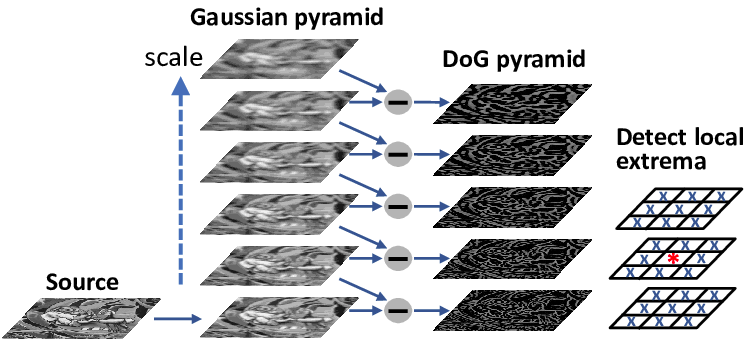
\includegraphics[width=0.8\linewidth]{DoG.png}
\end{center}

\section{Inverse Problems}

\subsection{Blur Models and Naive Inverse Filtering}

\begin{defbox}[title={Image Degradation Model}]
We observe a blurry, noisy image $y$. We want to recover the sharp original $x$.
Model: $y = x*h + \text{noise}$ where $h$ is the Point Spread Function (blur kernel).
\end{defbox}

\begin{thmbox}[title={Naive Inverse Filtering}]
Since spatial convolution is Fourier multiplication ($Y = X \cdot H + N$), the naive approach is:
\[
\hat{X} = \frac{Y}{H} = X + \frac{N}{H}.
\]
\textbf{Why this fails:} blur kernels $H$ destroy high frequencies, meaning $H \approx 0$ for high frequencies.
Dividing the noise $N$ by near-zero values causes $N/H$ to \textbf{explode}, burying the image in amplified noise.
\end{thmbox}

\subsection{Regularization}

\begin{intbox}
\textbf{Regularization} stabilizes inversion by trading off data fidelity and smoothness/prior assumptions.
Instead of dividing by tiny $H$, problematic frequencies are damped.
\end{intbox}

Classical options (know the idea and when they are used):
\begin{itemize}
  \item \textbf{Wiener filter:} frequency-dependent trade-off using noise/signal statistics.
  \item \textbf{Regularized filters:} add penalties (e.g., Tikhonov) to avoid unstable solutions.
  \item \textbf{Lucy--Richardson:} iterative deconvolution (often for Poisson noise).
  \item \textbf{Blind deconvolution:} estimate both $x$ and $h$ simultaneously (needs priors/constraints).
\end{itemize}

\section{Gradient-Domain Processing}

\subsection{Gradients as a Vector Field}

\begin{defbox}[title={Gradient Field}]
The image gradient field
\[
\vct{v} = (I_x, I_y)
\]
can be seen as a \textbf{vector field} over pixels.
If $\vct{v}$ is exactly the gradient of some image, it is \textbf{integrable} (conservative) with discrete curl $\approx 0$.
\end{defbox}

After editing a gradient field (e.g., mixing gradients from different images), it typically becomes non-conservative
(non-zero curl), so direct integration fails.

\subsection{Poisson Reconstruction}

\begin{thmbox}[title={Poisson Reconstruction}]
Given a desired vector field $\vct{v}=(v_x,v_y)$, recover an image $I$ whose gradients match $\vct{v}$
in least-squares sense:
\[
\min_I \sum_{m,n} \|\nabla I[m,n] - \vct{v}[m,n]\|^2
\quad\Longrightarrow\quad
\Delta I = \nabla\cdot \vct{v},
\]
a 2D Poisson equation with boundary conditions.
\end{thmbox}

The Laplacian $\Delta I$ is the divergence of the gradient, so it naturally appears in the normal equations.
Think of this as: \emph{choose the image whose gradients are as close as possible to what we want.}

Common gradient-domain applications:
\begin{itemize}
  \item \textbf{Seamless blending (Poisson blending):} paste an object while matching surrounding gradients.
  \item \textbf{Image fusion / reflection removal:} keep strong gradients from the desired layer, suppress others.
  \item \textbf{Stitching/editing:} reduce seams by enforcing consistent gradients across overlaps.
  \item \textbf{HDR/tone manipulation:} modify gradient magnitudes to compress dynamic range while preserving structure.
\end{itemize}

\section{CNN Note: Transposed Convolution}

\begin{thmbox}[title={Transposed Convolution (Learned Upsampling)}]
Often called ``deconvolution'', it is \emph{not} the inverse of a convolution, but a convolution applied to
an artificially inflated input.
\begin{enumerate}
  \item \textbf{Stretch:} insert $s-1$ zeros between every pixel (where $s$ is the stride).
  \item \textbf{Pad:} adjust the edges by subtracting padding $2p$.
  \item \textbf{Convolve:} slide a standard kernel of size $k$ over this new sparse grid.
\end{enumerate}
\textbf{Output size:}
\[
\text{out} = (\text{in}-1)\cdot s - 2p + k.
\]
\end{thmbox}


% ==========================================================
%  CHAPTER 4 — MACHINE LEARNING
% ==========================================================
\chapter{Machine Learning}

Training a model means choosing (i) a hypothesis space/model class, (ii) an objective/loss,
and (iii) an optimizer. Deep learning shifts much of the feature-design burden into learning,
but these three choices still matter in practice.

\section{Dimensionality Reduction}

High-dimensional image and feature vectors often lie near a lower-dimensional manifold or subspace.
Reducing dimensionality can: (i) denoise, (ii) compress, (iii) make learning easier with less overfitting,
and (iv) enable visualization.

\begin{intbox}
\textbf{Geometric picture:} find a low-dimensional subspace such that when you project the data onto it,
the projected points are still ``spread out'' as much as possible.
\end{intbox}

\subsection{Principal Component Analysis}

\begin{thmbox}[title={PCA Recipe}]
Goal: find a new set of axes (directions) that maximize the variance/spread of the data.
\begin{enumerate}
  \item \textbf{Center the data:} subtract the mean $\bar{\vct{x}}$ from all data points.
  \item \textbf{Covariance:} compute the covariance matrix $\mat{C} = \frac{1}{n}\mat{X}^\top\mat{X}$.
  \item \textbf{Eigen-decomposition:} find the eigenvectors and eigenvalues of $\mat{C}$.
\end{enumerate}
\textbf{Eigenvectors} are the new axes (Principal Directions); \textbf{eigenvalues} give the variance along each axis.
\textbf{Dimensionality reduction:} sort eigenvectors by highest eigenvalue and keep only the top-$k$.
\end{thmbox}

\subsection{Eigenfaces}

Flatten an $N\times M$ image into a vector in $\R^{NM}$. PCA on a set of face images yields a mean face
$\bar{\vct{x}}$ and eigenfaces $\{\vct{v}_1,\dots,\vct{v}_k\}$ (principal directions).

\begin{thmbox}[title={Projection and Reconstruction}]
\[
\vct{a} = \mat{V}_k^\top (\vct{x}-\bar{\vct{x}}),
\qquad
\hat{\vct{x}} = \bar{\vct{x}} + \mat{V}_k \vct{a},
\]
where $\mat{V}_k=[\vct{v}_1,\dots,\vct{v}_k]$.
\end{thmbox}

\begin{exbox}[title={Recognition via Eigenfaces}]
Project a test face to PCA coefficients $\vct{a}$ and do nearest-neighbor matching in coefficient space.
Works if training variation matches test variation; fails under large changes in illumination, pose, or expression.
\end{exbox}

The claim that ``Eigenface-based recognition is highly robust to extreme lighting/pose/expression changes''
is \textbf{incorrect} --- this is a common exam trap.

\section{Deep Learning for Images: CNN Essentials}

\subsection{Convolution Layer Computation}

A convolution layer applies $K$ learned filters to an input tensor $\mat{X}\in\R^{H\times W\times C}$.

\begin{thmbox}[title={How a Filter Works (3D Sliding Dot Product)}]
For each position in the image:
\begin{enumerate}
  \item \textbf{Extract a 3D patch:} take a chunk of the image that matches the filter's spatial size ($k \times k$) across \emph{all} input channels $C$.
  \item \textbf{Dot Product:} multiply every patch value with the corresponding filter weight and sum into a single number.
  \item \textbf{Add Bias:} add a learned scalar bias $b$.
\end{enumerate}
Sliding the same filter over the whole image gives \textbf{translation equivariance}.
\end{thmbox}

\begin{center}
  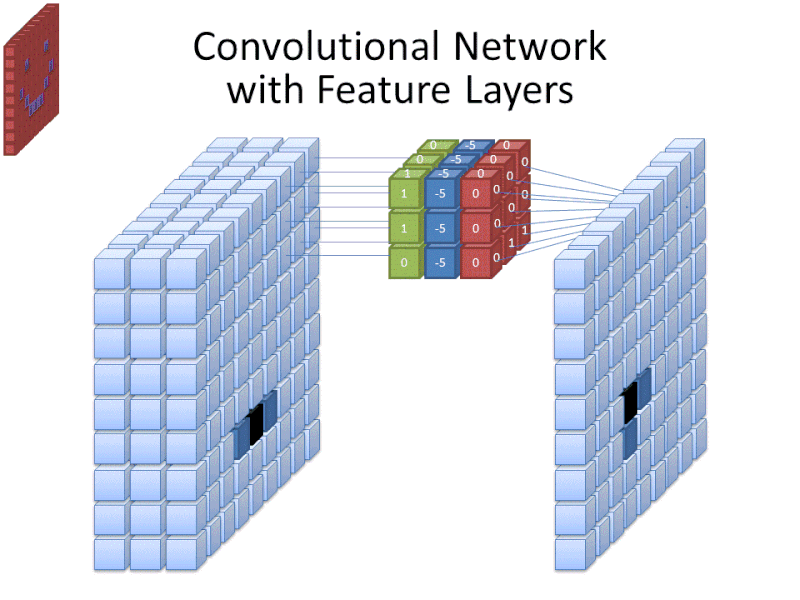
\includegraphics[width=0.5\linewidth]{3d_conv.png}
\end{center}

\begin{thmbox}[title={CNN Dimensions and Parameters}]
\textbf{Output Spatial Size:}
\[
\text{Size}_{\text{out}} = \Big\lfloor\frac{\text{Size}_{\text{in}} + 2 \times \text{padding} - \text{kernel\_size}}{\text{stride}}\Big\rfloor + 1
\]

\textbf{Number of Parameters (Weights):}
\[
\text{Params} = (\text{kernel\_width} \times \text{kernel\_height} \times \text{Channels}_{\text{in}} + 1) \times \text{Filters}_{\text{out}}
\]
(The $+1$ accounts for bias per filter.)
\end{thmbox}

\begin{exbox}[title={CNN Dimension Calculation}]
\textbf{Size:} Input $32\times 32$, $7\times 7$ conv, $s=1, p=0 \Rightarrow 26\times 26$. Three such layers: $32 \to 26 \to 20 \to 14$.\\
\textbf{Params:} Input has 3 channels, 16 filters of size $3\times 3$ (no bias). Each filter has $3 \times 3 \times 3 = 27$ weights. Total: $16 \times 27 = 432$.
\end{exbox}

\subsection{Nonlinearities, Pooling, and Receptive Field}

\begin{defbox}[title={ReLU and Pooling}]
\begin{itemize}
  \item \textbf{ReLU:} $f(x)=\max(0,x)$ introduces non-linearity and sparsity.
  \item \textbf{Pooling (e.g., max-pool):} downsamples feature maps; increases robustness to small translations,
  reduces computation, and increases receptive field.
\end{itemize}
\end{defbox}

\begin{itemize}
  \item \textbf{Stride:} step size of the kernel; larger stride produces downsampling.
  \item \textbf{Padding:} how boundaries are handled; ``same'' padding keeps spatial resolution.
  \item \textbf{Receptive field:} region of input that influences one output activation; grows with depth and pooling.
\end{itemize}

Convolution gives \emph{translation equivariance}, not full translation invariance.
Pooling and aggregation is what increases invariance to small shifts --- a common exam point.

\subsection{Classifier Head and Dense Prediction}

A typical classifier CNN ends with: spatial aggregation (flatten or global average pooling),
fully connected layer(s), then class scores (logits) fed to softmax probabilities.

A convolution kernel computes a weighted sum over a local patch and produces a strong response
where the patch matches the kernel. This can be used not only for whole-image classification but also for
\emph{dense} prediction --- predicting the class of the center pixel from its neighborhood.
This viewpoint connects CNNs naturally to semantic segmentation.


% ==========================================================
%  CHAPTER 5 — FEATURE EXTRACTION
% ==========================================================
\chapter{Feature Extraction}

Early visual processing decomposes input into features (color differences, local edges/textures, motion);
higher-level perception groups them into contours and regions. Good features are the foundation of
matching, retrieval, and recognition pipelines.

\section{What Makes a Good Feature?}

\begin{defbox}[title={Properties of Good Local Features}]
A good local feature is:
\begin{itemize}
  \item \textbf{Repeatable:} detected at the same physical scene point across views/conditions.
  \item \textbf{Distinctive:} descriptor discriminates it from others (few false matches).
  \item \textbf{Robust:} stable under noise, blur, illumination changes, and modest viewpoint changes.
  \item \textbf{Efficient:} computable and matchable at scale.
\end{itemize}
\end{defbox}

\section{Model-Based vs.\ Learning-Based Feature Extraction}

The classic local-feature pipeline is:
\[
\text{detect keypoints} \ \rightarrow\ \text{compute descriptor}\ \rightarrow\ \text{match descriptors}.
\]
Used in registration, panorama stitching, Structure from Motion (SfM), and retrieval.
Instead of manually designing kernels and descriptors, CNNs learn filter banks from data via backpropagation,
producing task-adapted features for classification, detection, or segmentation.

\subsection{Bag of Visual Words}

\begin{thmbox}[title={BoVW Pipeline}]
Represent the whole image as a frequency histogram of ``visual words'':
\begin{enumerate}
  \item \textbf{Extract:} find keypoints and compute local descriptors (e.g., SIFT) across all training images.
  \item \textbf{Build Vocabulary:} group all descriptors into $K$ clusters using $k$-means; cluster centers are ``visual words''.
  \item \textbf{Encode Image:} for a new image, assign each descriptor to the nearest visual word (hard assignment).
  \item \textbf{Pool:} count frequencies of each word to form a single $K$-dimensional histogram.
  \item \textbf{Classify:} feed the histogram vector into a standard classifier (e.g., SVM).
\end{enumerate}
\end{thmbox}

This is a useful conceptual bridge to CNNs, which \emph{learn} filters end-to-end and also use pooling to gain robustness.

\section{Invariances}

Scale changes are ubiquitous (objects at different distances). Many hand-crafted filters are translation-equivariant
detectors (Gaussian smoothing, derivatives, Laplacian). In CNNs, learned convolution kernels provide
translation-equivariant feature extraction. For scale, the classic solution is \textbf{explicit multi-scale}
processing (pyramids and scale space).

\section{SIFT (Scale-Invariant Feature Transform)}

\subsection{The SIFT Pipeline}

\begin{enumerate}
  \item \textbf{Scale space (DoG):} build Gaussian pyramid and compute Difference-of-Gaussians to approximate LoG.
  \item \textbf{Keypoint detection:} find local extrema of DoG in 3D neighborhood (space + scale).
  \item \textbf{Filtering:} reject low-contrast (noise) and unstable (edge) points.
  \item \textbf{Orientation assignment:} find dominant gradient orientation peak to normalize rotation.
  \item \textbf{Descriptor construction:} take patch aligned to orientation, split into $4\times4$ tiles. Build 8-bin gradient histogram per tile $\Rightarrow \mathbf{128\text{-D}}$ descriptor. Normalize for illumination.
\end{enumerate}

\begin{notebox}[title={SIFT Invariances and Limitations}]
SIFT is robust to \textbf{(i)} translation (locality), \textbf{(ii)} scale (scale space),
\textbf{(iii)} rotation (orientation assignment), and moderately to illumination (normalization).
It is \emph{not} fully invariant to large viewpoint changes or heavy blur/occlusion.
\end{notebox}

Match by nearest neighbor (Euclidean distance). The ratio test (best vs.\ second-best distance)
helps reject ambiguous matches. Failure modes: repetitive textures, large viewpoint changes, significant appearance changes.

\section{CNN Features as Descriptors}

Intermediate activations of a CNN serve as features at different levels of abstraction:
\begin{itemize}
  \item Early layers: edges and textures (low-level). Exam fact: here you expect to find learned filter kernels that approximate Gaussians.
  \item Middle layers: parts and patterns (mid-level).
  \item Deep layers: semantic concepts (high-level).
\end{itemize}

Architecture milestones:
\begin{itemize}
  \item \textbf{AlexNet (2012):} established modern deep CNNs for large-scale classification.
  \item \textbf{VGG (2014):} deeper stacks of small ($3\times3$) convolutions.
  \item \textbf{GoogLeNet/Inception (2015):} multi-branch modules for efficiency.
  \item \textbf{ResNet (2016):} residual connections enable very deep networks.
\end{itemize}

\begin{notebox}[title={Top-5 Error Rate}]
A prediction is counted as correct if the true label is among the top-5 predicted classes (so \emph{error} means it is not in the top 5).
Exam fact: ResNet can achieve a better top-5 error rate than humans.
\end{notebox}


% ==========================================================
%  CHAPTER 6 — SEGMENTATION
% ==========================================================
\chapter{Segmentation}

Segmentation partitions an image into groups of pixels that belong together, assigning a label to every pixel
rather than a single label for the whole image. It is fundamental to image editing, autonomous driving,
and medical imaging.

\section{What is Segmentation?}

\begin{defbox}[title={Segmentation}]
\textbf{Segmentation} = partition an image into \textbf{groups of pixels that belong together}.
The output is a label per pixel (a mask).
\begin{itemize}
  \item \textbf{Semantic segmentation:} assigns a \emph{class label} to every pixel (all ``car'' pixels share the same label).
  \item \textbf{Instance segmentation:} separates \emph{individual object instances} (car \#1 vs.\ car \#2).
  \item \textbf{Panoptic segmentation:} combines both: semantic classes \emph{and} instance IDs where applicable.
\end{itemize}
\end{defbox}

Classification has no spatial extent; detection outputs boxes; segmentation outputs pixel masks.
Do not confuse \emph{semantic segmentation} (pixel-wise class labels) with \emph{instance segmentation} (separate object IDs) --- a common exam pitfall.

Segmentation is hard because boundaries may be weak or blurred, objects can have similar color/texture,
and occlusions hide parts. Dense pixel labels are also expensive to annotate.

\section{Segmentation by Clustering}

Pixels can be modeled as points in feature space and clustered. Typical feature choices:
color only ($\vct{x}_i = (R_i,G_i,B_i)\in\R^3$) or color + location
($\vct{x}_i = (R_i,G_i,B_i,u_i,v_i)\in\R^5$, which encourages spatial coherence).
Adding $(u,v)$ helps avoid grouping distant pixels that merely share color; normalize color vs.\ position
so neither dominates distances.

\subsection{K-Means Clustering}

\begin{defbox}[title={K-Means}]
\textbf{$k$-means} partitions $\{\vct{x}_i\}_{i=1}^N$ into $k$ clusters by minimizing within-cluster squared distances.
\end{defbox}

\begin{thmbox}[title={K-Means Objective}]
\[
\min_{\{\mathcal{C}_1,\dots,\mathcal{C}_k\}} \ \sum_{c=1}^k \sum_{i\in\mathcal{C}_c} \|\vct{x}_i - \vct{\mu}_c\|^2,
\qquad
\vct{\mu}_c = \frac{1}{|\mathcal{C}_c|}\sum_{i\in\mathcal{C}_c}\vct{x}_i.
\]
\end{thmbox}

Algorithm: (1) initialize $k$ cluster centers; (2) assign each point to nearest center;
(3) recompute centers as cluster means; (4) repeat until convergence.

Typical failure modes: must choose $k$ in advance; sensitive to initialization (local minima); not boundary-aware
(can ``bleed'' across edges).

\section{Segmentation with Graphs}

\begin{defbox}[title={Graph-Based Segmentation}]
Build a graph $G=(V,E)$ where nodes are pixels (or superpixels) and edges connect neighbors with affinity weights
encoding similarity. Affinity weight $a_{ij}$ is large if pixels are similar in color and close in space.
\end{defbox}

\subsection{Spectral Clustering}

\begin{thmbox}[title={Spectral Clustering}]
Instead of clustering in coordinate space, cluster based on graph connectivity:
\begin{enumerate}
  \item \textbf{Affinity Matrix ($\mat{A}$):} $A_{ij}$ is high if pixel $i$ and $j$ are similar.
  \item \textbf{Goal:} find a group assignment vector $\vct{w}$ maximizing connections within the group: $\max (\vct{w}\T \mat{A}\vct{w})$.
  \item \textbf{Solution:} maximizing this quadratic form (normalized $\vct{w}$) is solved by the \textbf{eigenvectors} of $\mat{A}$ (or the Graph Laplacian) corresponding to the largest eigenvalues.
\end{enumerate}
\end{thmbox}

When iteratively extracting one cluster per round and stopping when the largest eigenvalue drops below a threshold:
$\#\text{clusters} = \#\{\text{rounds with } \lambda_{\max} \ge \text{threshold}\}$.

\subsection{Graph Cut and GrabCut}

\begin{thmbox}[title={Graph Cut Energy Minimization}]
Assign a label $y_i$ (foreground or background) to each pixel to minimize:
\[
E(\vct{y}) = \underbrace{\sum_i D_i(y_i)}_{\text{Data term}} \;+\; \lambda \underbrace{\sum_{(i,j)\in E} V_{ij}(y_i,y_j)}_{\text{Smoothness term}}
\]
\begin{itemize}
  \item \textbf{Data term:} cost of assigning a pixel to a label (does it look like foreground or background?).
  \item \textbf{Smoothness term:} penalizes different labels for neighboring pixels unless there is a strong natural edge.
\end{itemize}
The global optimum is found efficiently via \textbf{min-cut/max-flow} algorithms.
\end{thmbox}

\textbf{GrabCut} is an interactive tool using Graph Cuts: the user draws a bounding box; the algorithm builds
Gaussian Mixture Models (GMMs) for foreground/background, runs min-cut, updates the GMMs, and repeats iteratively.

\section{Segmentation by Fitting}

\subsection{Hough Transform}

If segments correspond to known parametric shapes (lines, circles, etc.), detect them by searching in the
\textbf{parameter space} of that shape family.

\begin{defbox}[title={Hough Transform}]
A voting scheme: edge pixels vote for shape parameters; peaks in an accumulator array indicate shapes.
\end{defbox}

\begin{thmbox}[title={Line Parameterization}]
\[
\rho = x\cos\theta + y\sin\theta.
\]
Each edge pixel $(x,y)$ votes for all $(\rho,\theta)$ pairs consistent with it.
\end{thmbox}

Procedure: (1) run edge detector; (2) each edge pixel votes in accumulator $H(\rho,\theta)$;
(3) find peaks above threshold; (4) convert peak parameters back to image lines.

The Hough space dimension equals the number of free shape parameters:
2D line: 2 parameters $(\rho,\theta)$; 2D circle: 3 parameters $(x_0,y_0,r)$;
2D ellipse: \textbf{5 parameters} $(x_0,y_0,a,b,\theta)$; 3D ellipsoid: typically \textbf{9 parameters}.
More parameters means a larger accumulator and higher computational cost.

\section{Segmentation by Learning}

\subsection{Fully Convolutional Networks}

\begin{defbox}[title={Learning-Based Semantic Segmentation}]
Uses \textbf{paired training data}: for each training image, every pixel has a class label.
At test time, the model predicts a label for every pixel.
\end{defbox}

\begin{thmbox}[title={FCN Score-Tensor View}]
\[
\underbrace{3\times H\times W}_{\text{input}}
\ \xrightarrow{\text{encoder (down)}}\
\underbrace{C\times H'\times W'}_{\text{scores}}
\ \xrightarrow{\text{decoder (up)}}\
\underbrace{C\times H\times W}_{\text{scores}}
\ \xrightarrow{\argmax}\
\underbrace{H\times W}_{\text{labels}}.
\]
\end{thmbox}

Classification CNNs downsample aggressively to gain receptive field and efficiency,
but segmentation needs \textbf{dense output at input resolution}. Two strategies:
no downsampling (expensive) or encoder--decoder (downsample then upsample).

\subsection{U-Net and Skip Connections}

\begin{defbox}[title={U-Net}]
Plain encoder--decoder (autoencoder) can produce blurry or imprecise boundaries because fine spatial detail is lost.
\textbf{U-Net} improves this via \textbf{skip connections} that pass high-resolution encoder features directly to the decoder.
\end{defbox}

Skip connections let the decoder combine: \textbf{(i)} global semantic understanding (deep, low-resolution features)
with \textbf{(ii)} local detail (shallow, high-resolution features), yielding sharper masks.

A \textbf{1$\times$1 convolution} performs a learned linear map $\R^{D}\to\R^{C}$ per pixel independently.
Uses: project feature depth $D$ to number of classes $C$ (per-pixel score maps), or bottlenecking for efficiency.


% ==========================================================
%  CHAPTER 7 — OPTICAL FLOW
% ==========================================================
\chapter{Optical Flow}

Optical flow captures apparent motion in image sequences. It is the foundation of video compression,
tracking, action recognition, and autonomous driving perception.

\section{Definition and Use Cases}

\begin{defbox}[title={Optical Flow}]
\textbf{Optical flow} estimates the apparent \textbf{2D motion field} between two consecutive frames:
each pixel (or region) is assigned a displacement vector $(u,v)$ from time $t$ to $t+1$.
\begin{itemize}
  \item \textbf{Sparse flow:} vectors only at selected points/patches (fast; relies on good features).
  \item \textbf{Dense flow:} vector for every pixel (useful for motion segmentation, tracking, video understanding).
\end{itemize}
\end{defbox}

Common use cases: video compression (motion-compensated prediction), tracking and action recognition,
robotics and autonomous driving, and medical/scientific imaging (deformation fields, registration).
Flow fields are often visualized with a \textbf{color wheel}: direction maps to hue, magnitude to saturation/brightness.

\begin{notebox}[title={Stereo Connection}]
For a static rectified stereo-camera system and a static scene, the dense optical flow field correlates directly to a disparity map.
\end{notebox}

\section{Core Assumptions}

Three assumptions underlie classical optical flow methods:
\begin{itemize}
  \item \textbf{Brightness constancy} (photometric consistency).
  \item \textbf{Small motion} (enables Taylor linearization), handled for larger motion via pyramids/warping.
  \item \textbf{Spatial coherence} / \textbf{locally constant flow} in a small window.
\end{itemize}

\begin{defbox}[title={Brightness Constancy}]
\[
I(x,y,t)\approx I(x+u,\,y+v,\,t+1).
\]
\end{defbox}

Brightness constancy breaks under illumination changes, specularities, motion blur, and occlusions.
Smoothness assumptions can oversmooth across motion boundaries.

\section{Optical Flow Constraint Equation}

\subsection{Derivation}

Starting from $I(x+u,y+v,t+1)\approx I(x,y,t)$ and applying a first-order Taylor expansion:

\begin{thmbox}[title={Optical Flow Constraint Equation (OFCE)}]
\[
I_x\,u + I_y\,v + I_t = 0,
\]
where $I_x,I_y$ are spatial derivatives and $I_t$ is the temporal derivative.
\end{thmbox}

\subsection{Aperture Problem}

\begin{defbox}[title={Aperture Problem}]
The OFCE provides \emph{one equation} for two unknowns $(u,v)$ at each pixel.
Along an edge, only motion \emph{normal to the edge} is constrained; tangential motion is ambiguous.
\end{defbox}

\section{Classical Methods}

\subsection{Lucas--Kanade (Local Window)}

\begin{thmbox}[title={Lucas-Kanade Solution}]
\begin{enumerate}
  \item \textbf{Assumption:} assume flow $(u,v)$ is identical for all pixels in a small window (e.g., $3 \times 3$).
  \item \textbf{Overdetermined System:} 9 equations, 2 unknowns.
  \item \textbf{Least Squares:} solve for the best-fitting $(u,v)$.
\end{enumerate}
\textbf{Crucial Condition:} this only works if the window has gradients in at least two different directions
(i.e., it must be a \textbf{corner}, not a flat region or a single straight edge).
\end{thmbox}

\subsection{Coarse-to-Fine for Large Motion}

If motion exceeds approximately 1 pixel, the linearization breaks. The standard fix is \textbf{coarse-to-fine estimation}:

\begin{enumerate}
  \item Build Gaussian pyramids of both frames.
  \item Estimate flow at the coarsest level.
  \item \textbf{Upsample flow}, \textbf{warp} the second image toward the first, and refine at the next finer level.
  \item Repeat until full resolution.
\end{enumerate}

\subsection{Horn--Schunck (Global Energy)}

\begin{thmbox}[title={Horn--Schunck Global Energy}]
Compute flow for \emph{every} pixel simultaneously by minimizing:
\[
E = E_{\text{data}} + \lambda E_{\text{smooth}}
\]
\begin{itemize}
  \item \textbf{Data term ($E_{\text{data}}$):} penalizes deviations from brightness constancy (the OFCE).
  \item \textbf{Smoothness term ($E_{\text{smooth}}$):} penalizes differences between neighboring flow vectors.
\end{itemize}
\end{thmbox}

The parameter $\lambda$ controls the trade-off. A larger $\lambda$ forces a smoother flow field but risks
washing out sharp motion boundaries where two objects move past each other.

\section{Optical Flow and Learning}

\begin{defbox}[title={Learning-Based Flow}]
Learning-based flow models treat optical flow as a supervised prediction task:
input = two frames, output = dense flow field (often via an encoder--decoder/U-Net-like design).
\end{defbox}

Deep methods learn a \textbf{direct mapping} from an image pair to a dense flow field.
They do \textbf{not} require explicit hand-computed image gradients at inference time.

FlowNet variants from the lecture:
\begin{itemize}
  \item \textbf{FlowNetS (Simple):} stack two RGB images into one input tensor and predict flow end-to-end.
  \item \textbf{FlowNetCorr (Correlation):} compute feature maps per image, then use a \textbf{correlation layer}
        to explicitly match features before decoding to flow.
\end{itemize}

\begin{notebox}[title={Exam Trap}]
Typical failure cases for both classical and learned flow:
occlusions (no correspondence), large displacements without enough pyramid/context,
illumination changes (brightness constancy violated), and motion boundaries (smoothness vs.\ sharp edges).
\end{notebox}


% ==========================================================
%  CHAPTER 8 — OBJECT DETECTION
% ==========================================================
\chapter{Object Detection}

Object detection must answer not just \emph{what} is in an image but \emph{where} it is.
Detection is harder than classification because the output size is variable (unknown number of objects)
and the model must jointly handle \textbf{localization} and \textbf{classification}.

\section{Problem Setup}

\begin{itemize}
  \item \textbf{Image classification:} output a single (or multi-) label for the whole image.
  \item \textbf{Single-object detection:} predict class + one bounding box for the dominant object.
  \item \textbf{Multi-object detection:} predict a \emph{set} of objects, each with class + bounding box (optionally a mask).
\end{itemize}

\begin{defbox}[title={Bounding Box}]
A \textbf{bounding box} is typically parameterized as
\[
(x, y, w, h) \quad \text{or} \quad (x_{\min}, y_{\min}, x_{\max}, y_{\max}),
\]
plus a \textbf{confidence score} and a \textbf{class label}.
\end{defbox}

\begin{thmbox}[title={Multi-Task Detection Loss}]
\[
\mathcal{L} = \mathcal{L}_{\text{cls}} + \lambda\,\mathcal{L}_{\text{box}} \ (+\ \mathcal{L}_{\text{mask}} \text{ for instance segmentation}),
\]
e.g.\ cross-entropy for classes and a regression loss for boxes.
\end{thmbox}

Localization is treated as a \emph{regression problem} (predicting box coordinates), not classification.

\section{Region Proposals and the R-CNN Family}

\subsection{Selective Search and R-CNN}

\begin{defbox}[title={Region Proposals}]
\textbf{Region proposals} are candidate image regions likely to contain an object.
\textbf{Selective Search} generates proposals by hierarchical grouping of superpixels using similarity cues
(color, texture, size, fill).
\end{defbox}

R-CNN: generate region proposals, then for each proposal warp/crop $\rightarrow$ CNN $\rightarrow$ classify and refine box.
Conceptually simple but inefficient: it runs a CNN \emph{many times} per image (once per proposal).

\subsection{Fast R-CNN and Faster R-CNN}

\begin{defbox}[title={Fast R-CNN}]
Run a CNN \emph{once} on the whole image to get a feature map, then extract fixed-size features per proposal via
\textbf{RoI pooling} (or RoIAlign in later variants).
Shared convolutional backbone makes it much faster than R-CNN, but still relies on external proposals.
\end{defbox}

\begin{defbox}[title={Region Proposal Network (RPN)}]
\textbf{Faster R-CNN} replaces external proposals with an RPN that learns proposals directly from the shared feature map.
At each spatial location it predicts: \textbf{(i)} an objectness score and \textbf{(ii)} box transforms for multiple anchors.
\end{defbox}

\subsection{Anchors and Bounding-Box Regression}

\begin{defbox}[title={Anchors}]
\textbf{Anchors} are predefined reference boxes (multiple scales/aspect ratios) centered at each feature-map location.
The network predicts offsets that transform an anchor into the final box.
\end{defbox}

\begin{thmbox}[title={Anchor Offset Parameterization}]
For anchor $(x_a,y_a,w_a,h_a)$ and target $(x,y,w,h)$:
\[
t_x=\frac{x-x_a}{w_a},\quad t_y=\frac{y-y_a}{h_a},\quad
t_w=\log\frac{w}{w_a},\quad t_h=\log\frac{h}{h_a}.
\]
The model predicts $(t_x,t_y,t_w,t_h)$.
\end{thmbox}

More anchors gives better coverage but more class imbalance (many negatives).

\subsection{Mask R-CNN}

\begin{defbox}[title={Mask R-CNN}]
Extends Faster R-CNN with a parallel \textbf{mask head} that predicts a binary mask for each detected RoI,
yielding \textbf{instance segmentation}: a mask per object instance.
Detection head: class + bounding box. Mask head: per-RoI pixelwise mask (e.g.\ $28\times 28$) for the predicted class.
\end{defbox}

\section{Single-Shot Detectors}

Single-shot means: one forward pass produces class scores and boxes densely over the image with no explicit proposal stage.

\begin{itemize}
  \item \textbf{YOLO:} grid-based prediction; very fast, historically struggles with small objects (varies by version).
  \item \textbf{SSD:} multi-scale feature maps + default boxes (anchors) at different resolutions.
  \item \textbf{RetinaNet:} single-shot with \textbf{focal loss} to address extreme foreground/background imbalance.
\end{itemize}

\begin{defbox}[title={YOLO}]
Splits the image into an $S\times S$ grid. The \textbf{cell containing the object center} is responsible for predicting it.
Per cell it predicts $B$ boxes and class scores.
\[
Y = [p_c,\ b_x,\ b_y,\ b_w,\ b_h,\ c_1,\dots,c_C],
\]
where $p_c$ is objectness/confidence, $(b_x,b_y,b_w,b_h)$ are box parameters, and $c_k$ are class scores.
The full output tensor for YOLOv1-style models is $S\times S\times (5B + C)$.
\end{defbox}

\subsection{IoU and Non-Maximum Suppression}

\begin{thmbox}[title={Intersection over Union}]
\[
\mathrm{IoU}(A,B)=\frac{\mathrm{area}(A\cap B)}{\mathrm{area}(A\cup B)}\in[0,1].
\]
\end{thmbox}

\begin{defbox}[title={Non-Maximum Suppression (NMS)}]
Reduces duplicate detections: keep the highest-confidence box and suppress other boxes with IoU above a threshold, then repeat.
\begin{enumerate}
  \item Sort predicted boxes by confidence (descending).
  \item Take the top box; remove all remaining boxes with $\mathrm{IoU}>\tau$ to it.
  \item Repeat until no boxes remain.
\end{enumerate}
\end{defbox}

IoU is used both for \emph{training/label assignment} (which predictions match a GT box) and for
\emph{post-processing NMS} to remove duplicates --- these are two separate uses.

Dense detectors evaluate many candidate boxes, most of which are background. Standard cross-entropy can be
dominated by easy negatives. \textbf{Focal loss} down-weights easy examples so the model focuses on hard,
informative mistakes.

\section{Evaluation}

\begin{defbox}[title={Detection Evaluation Basics}]
Standard precision/recall metrics are used, but a True Positive (TP) requires:
\begin{itemize}
  \item \textbf{TP:} correct class AND bounding box overlaps Ground Truth by \textbf{IoU > threshold} (e.g., 0.5).
  \item \textbf{FP:} IoU too low, wrong class, or a duplicate.
  \item \textbf{FN:} an actual object was missed.
\end{itemize}
\end{defbox}

Varying the confidence threshold yields a \textbf{Precision--Recall curve}.
A better detector has a curve closer to the top-right corner (high precision at high recall).

\begin{defbox}[title={AP and mAP}]
\textbf{Average Precision (AP)} is the area under the Precision--Recall curve for a class.
\textbf{mAP} is the mean AP over all classes (and sometimes over multiple IoU thresholds).
\end{defbox}

\section{Vision Transformers}

CNNs have a strong \textbf{locality} and \textbf{translation-equivariance} bias.
Transformers model \textbf{global interactions} via attention, capturing long-range dependencies more directly.
Historically, transformers tend to be more data-hungry than CNNs unless pretrained at scale.

\begin{defbox}[title={Vision Transformer (ViT)}]
Split an image into fixed-size patches, embed each patch as a token, add positional encodings,
then apply a standard transformer encoder. A special \textbf{class token} can aggregate information for classification.
\end{defbox}


% ==========================================================
%  CHAPTER 9 — MULTI-VIEW GEOMETRY
% ==========================================================
\chapter{Multi-View Geometry}

A single image pixel corresponds to a \emph{ray} in 3D --- infinitely many 3D points are consistent with it.
With two or more views, rays from different camera centers intersect (approximately), making depth recoverable.
This chapter develops the geometry underlying stereo, feature matching, and Structure from Motion.

\section{Transformations (Exam Essentials)}

\begin{notebox}[title={Key Transforms}]
\textbf{Euclidean (rigid) transform:} rotation + translation; preserves distances and angles.\\
\textbf{Affine transform:} Euclidean + general linear transform (scaling, shear) + translation; preserves parallel lines, not angles/lengths.
\end{notebox}

\section{Recap: Camera Model Prerequisites}

\begin{thmbox}[title={Pinhole Camera Model}]
\[
\tilde{\vct{p}} \sim \mat{P}\,\tilde{\vct{P}}_W,
\qquad
\mat{P}=\mat{K}[\mat{R}\mid \vct{t}].
\]
\end{thmbox}

A $3\times 4$ camera matrix has 12 entries but is defined up to scale ($\Rightarrow 11$ DOF).
Each 3D--2D correspondence gives 2 independent equations, so at least \textbf{6} correspondences are needed (DLT).

\begin{defbox}[title={Normalized Image Coordinates}]
\[
\tilde{\vct{x}} \sim \mat{K}^{-1}\tilde{\vct{p}}
\]
removes the effect of intrinsics, placing points on a normalized (focal length $=1$) image plane.
\end{defbox}

Epipolar geometry is derived for the ideal pinhole model. In practice, \textbf{undistort} images (using calibration)
before estimating correspondences, $F/E$, disparity, etc.

\section{Feature Matching Across Views}

\begin{defbox}[title={Correspondences}]
A \textbf{correspondence} is a pair of image points $(\vct{p},\vct{p}')$ from the same 3D scene point.
Real matching produces \textbf{outliers} due to repeated texture, occlusions, specularities, and noise.
\end{defbox}

Use distinctive descriptors (e.g.\ SIFT) with nearest-neighbor matching, ratio test heuristics,
and robust estimation (RANSAC) to handle outliers.
Good sparse matches enable: estimating epipolar geometry ($F/E$), rectification, triangulation, and SfM pipelines.

\section{Epipolar Geometry}

\begin{defbox}[title={Epipolar Geometry}]
Imagine a triangle formed by Camera A, Camera B, and the 3D object point. This triangle defines the \textbf{epipolar plane}.
\begin{itemize}
  \item \textbf{Baseline:} the physical line connecting the two camera centers.
  \item \textbf{Epipoles:} what Camera A sees if it looks directly into the lens of Camera B (and vice versa).
  \item \textbf{Epipolar line:} the intersection of the epipolar plane with the camera's image sensor.
\end{itemize}
\end{defbox}

\begin{center}
  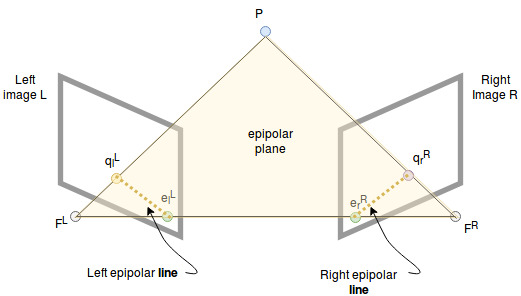
\includegraphics[width=0.7\linewidth]{epipolar.png}
\end{center}

The epipolar constraint means that to find a pixel's match in Image B, you only need to search along
a \textbf{specific epipolar line} (a fast 1D search) rather than the entire image (a 2D search).

\section{Essential and Fundamental Matrices}

\begin{thmbox}[title={E and F Relationship}]
\[
E = K_2^{\top} F K_1,
\qquad
F = K_2^{-\top} E K_1^{-1}.
\]
Use $F$ with \textbf{pixel} coordinates and $E$ with \textbf{normalized} coordinates.
One point $x$ in image 1 induces exactly \textbf{one} epipolar line $l_2 = F x$ in image 2.
\end{thmbox}

\begin{thmbox}[title={Epipolar Constraints}]
\textbf{Calibrated (normalized coordinates):}
\[
\tilde{\vct{x}}'^{\T}\,\mat{E}\,\tilde{\vct{x}} = 0.
\]
\textbf{Uncalibrated (pixel coordinates):}
\[
\tilde{\vct{p}}'^{\T}\,\mat{F}\,\tilde{\vct{p}} = 0.
\]
\end{thmbox}

In the calibrated case, $\mat{E}$ encodes the \textbf{relative pose} (up to scale) between the cameras.

Given $\mat{F}$, the epipolar line in image 2 for point $\tilde{\vct{p}}$ in image 1 is $\mat{\ell}' = \mat{F}\,\tilde{\vct{p}}$;
analogously, $\mat{\ell} = \mat{F}^{\T}\tilde{\vct{p}}'$ gives the line in image 1.

Estimation requires at least 8 correspondences (the classic \textbf{8-point algorithm}); more is better.
Use \textbf{RANSAC} to cope with outliers: repeatedly fit $\mat{F}/\mat{E}$ on minimal samples and keep the model with the most inliers.
Without robust estimation, a few bad matches can completely break estimation.

\section{Three-View Geometry}

A trifocal tensor can be represented as a $3\times3\times3$ array with \textbf{27 coefficients}
(it satisfies internal constraints; its DOF is smaller than 27).

\section{Rectification and Disparity}

\begin{defbox}[title={Rectification}]
\textbf{Rectification} warps the two images so that corresponding epipolar lines become \textbf{horizontal scanlines}.
Then correspondence search becomes a 1D search along image rows.
\end{defbox}

After rectification, a correspondence typically satisfies $y \approx y'$ and the remaining unknown is the horizontal shift.
\textbf{Disparity} is defined as $d = x_L - x_R$ (or opposite sign depending on convention).
Dense stereo estimates a disparity $d(x,y)$ for many/all pixels, producing a \textbf{disparity map}.

Learning-based stereo uses \textbf{cost volumes} built by combining left/right features across a range of disparities $d$,
yielding a volume of size $H\times W\times D$. A \textbf{3D CNN} then regularizes matching costs across $(x,y,d)$
and regresses the final disparity.

The \textbf{ordering constraint} (rectified stereo): along a scanline, the left-to-right order of corresponding points
is preserved for opaque non-occluded surfaces; violated by occlusions and repeated structures.

\section{Stereo Depth Reconstruction}

\begin{thmbox}[title={The Classic Stereo Formula}]
\[
Z = \frac{f \times B}{d}
\]
where $Z$ is depth, $f$ is focal length, $B$ is baseline (camera separation), and $d$ is disparity.
\begin{itemize}
  \item \textbf{To see further:} need larger baseline $B$ or larger focal length $f$.
  \item \textbf{Far-distance problem:} for distant objects $d \approx 0$; since $Z \propto 1/d$, a tiny 1-pixel matching error causes massive depth error.
\end{itemize}
\end{thmbox}

\begin{defbox}[title={Sparse vs.\ Dense Stereo}]
\textbf{Sparse stereo:} compute depth only at matched keypoints (robust, low density).
\textbf{Dense stereo:} estimate depth for (almost) every pixel using matching costs and regularization.
\end{defbox}

Dense stereo struggles in textureless regions, repetitive patterns, and at occlusion boundaries.

\section{Affine Structure from Motion}

\textbf{Affine shape:} reconstruction is defined only \textbf{up to an affine transformation}.
Two views of 4 non-coplanar points suffice to constrain affine shape; two views of 3 points do not.

A general affine camera is a $2\times4$ matrix (8 parameters per view).
With $m$ views and $n$ points, unknown coefficients $\approx 8m + 3n + 9$,
where the extra $+9$ reflects the inherent $3\times3$ affine ambiguity in factorization-based affine SfM.

\section{Structure from Motion (SfM)}

\begin{defbox}[title={SfM Pipeline}]
\textbf{SfM} generalizes stereo to \textbf{multiple} images: jointly estimate \textbf{camera poses} and \textbf{3D points}.
\[
\text{detect/match features} \rightarrow \text{estimate relative motion} \rightarrow \text{triangulate} \rightarrow \text{refine (bundle adjustment)}.
\]
\end{defbox}

\begin{itemize}
  \item Start from an initial image pair with good baseline.
  \item Incrementally add images: match to existing points, estimate new camera pose, triangulate new points.
  \item Refine by minimizing reprojection error (bundle adjustment).
\end{itemize}

\begin{notebox}[title={SfM Equation Counting ($m$ views, $n$ points)}]
Each 3D point gives 2 equations per view ($2mn$ equations total).

\textbf{Simple coefficient counting:} camera = 12 unknowns, point = 3 unknowns.
Solvable if: $2mn \ge 12m + 3n$.

\textbf{Projective DOF counting:} camera has 11 DOF, point has 3 DOF, coordinate system has 15-DOF ambiguity.
Solvable if: $2mn \ge 11m + 3n - 15$.
\begin{itemize}
  \item \textbf{2 Views ($m=2$):} needs $n > 7$ $\Rightarrow$ minimum \textbf{8 correspondences}.
  \item \textbf{3 Views / 3 Points:} $18 \ge 27$ $\Rightarrow$ \textbf{False} (not solvable).
\end{itemize}
\end{notebox}

SfM typically outputs camera poses for each image and a \textbf{sparse} 3D point cloud from feature tracks.
Absolute \textbf{scale} is ambiguous without additional information (known baseline, IMU, GPS, etc.).

Bad matches lead to wrong $\mat{F}/\mat{E}$, wrong rectification/triangulation, and broken reconstruction.
Robust matching and proper calibration/undistortion are essential.


% ==========================================================
%  CHAPTER 10 — 3D VISION
% ==========================================================
\chapter{3D Vision}

The previous chapters interpreted images as 2D signals (classification, segmentation, detection) and
recovered 3D structure from multiple views (stereo, SfM). This chapter focuses on how depth and shape
can be \emph{represented}, \emph{predicted} (often learning-based), and \emph{rendered} (NeRF).

\section{Depth from X}

\subsection{Depth from Stereo and Multiple Views}

\begin{defbox}[title={Depth from Stereo}]
Infer depth from \textbf{parallax} (viewpoint change). Matching corresponding points constrains depth;
larger baseline generally increases depth sensitivity.
\begin{itemize}
  \item \textbf{Stereo:} two calibrated views $\Rightarrow$ disparity $\Rightarrow$ depth (dense or sparse).
  \item \textbf{Multi-view / SfM:} many views $\Rightarrow$ estimate camera poses + sparse 3D points (then densify).
\end{itemize}
\end{defbox}

Classical stereo relies on: feature extraction, matching, geometry, and calibration.
Classical matching is brittle: pixel appearance depends on reflectance, shape, and shading,
but we only want shape, making correspondence (and thus depth) ill-posed in practice.

\subsection{Depth from Other Cues}

\begin{defbox}[title={Depth from X}]
Depth estimation using cues other than multi-view parallax, e.g.\ \textbf{shading} or \textbf{defocus}
(focus blur). Each cue requires additional assumptions about image formation.
\end{defbox}

Depth from defocus (DfD) requires \textbf{texture/high-frequency content}; in \textbf{uniform regions} blur is ambiguous.
CNN features (including early/mid conv layers) can correlate with focus/blur primarily in \textbf{non-uniform (textured)} regions.

\section{Depth Maps}

\begin{defbox}[title={Depth Map}]
A \textbf{depth map} stores one scalar per pixel: the distance from the camera to the observed surface point
along that pixel's viewing ray.
Together with RGB it forms an \textbf{RGB-D} image (often called ``2.5D'').
\end{defbox}

Depth maps are view-dependent: they represent only what is visible from the camera.
Depth can be captured directly by structured light or time-of-flight devices (e.g., Microsoft Kinect).

\subsection{Structured Light with Gray Codes}

\begin{notebox}[title={Gray Code Properties}]
Neighboring codewords differ by \textbf{Hamming distance 1} (only one bit changes), reducing decoding errors at boundaries.
For resolution $W\times H$, you need $\lceil\log_2 W\rceil$ patterns for columns and $\lceil\log_2 H\rceil$ for rows.
Example: $1024\times1024$ needs $10+10=\textbf{20}$ images.
\end{notebox}

\subsection{Light Transport and Helmholtz Reciprocity}

Model light transport as a linear map: camera image $c = T\,p$ (projector pattern $p$, transport matrix $T$).
\textbf{Helmholtz reciprocity} implies a swap of emitter/sensor corresponds to the \textbf{transpose} mapping ($T^\top$).
Thus \textbf{dual photography}: $p = T^\top c$.
If $c$ is uniform white, then $p$ visualizes the scene as seen from the projector viewpoint under uniform camera-side illumination.

\subsection{Evaluating Depth Maps}

Two common viewpoints:
\begin{itemize}
  \item \textbf{Per-pixel errors} between predicted and measured depth (after masking invalid pixels).
  \item \textbf{Log-depth errors} to reduce sensitivity to absolute scale and emphasize relative accuracy.
\end{itemize}

\begin{thmbox}[title={Per-Pixel Log-Depth Loss}]
Given ground truth $y_i$ and prediction $y_i^\ast$ at pixel $i$:
\[
D_{L2}(y,y^\ast) = \frac{1}{n}\sum_{i=1}^{n}\left(\log y_i - \log y_i^\ast\right)^2.
\]
\end{thmbox}

\subsection{Scale-Depth Ambiguity and Scale-Invariant Loss}

From a single image, \textbf{absolute scale} is fundamentally ambiguous without additional cues or priors ---
a small close object can produce the same image as a large far object.

\begin{thmbox}[title={Scale-Invariant Loss}]
\[
D_{SI}(y,y^\ast)=\frac{1}{n}\sum_{i=1}^{n}\left(\log y_i - \log y_i^\ast + \alpha(y,y^\ast)\right)^2,
\qquad
\alpha(y,y^\ast)=\frac{1}{n}\sum_{j=1}^{n}\left(\log y_j - \log y_j^\ast\right).
\]
$\alpha$ compensates a global scale offset in log-space (a global multiplicative depth scaling).
\end{thmbox}

\begin{defbox}[title={Monocular Depth Learning}]
Train a CNN that maps an RGB image ($3\times H\times W$) to a depth map ($1\times H\times W$) using paired training data
(RGB, measured depth) and a per-pixel loss.
Depth supervision can come from RGB-D sensors or from multi-view reconstruction pipelines.
\end{defbox}

\section{Surface Normals}

\begin{defbox}[title={Surface Normal Map}]
A \textbf{surface normal map} stores a 3D unit vector per pixel ($3\times H\times W$) describing local surface orientation
(perpendicular to the tangent plane).
\end{defbox}

Depth and normals are tightly related:
depth $\rightarrow$ normals via spatial derivatives (gradients of reconstructed surface);
normals $\rightarrow$ depth via integration (a PDE/reconstruction problem).

\begin{thmbox}[title={Angular Error for Normals}]
\[
\theta = \arccos\!\left(\frac{\vct{n}\cdot \vct{n}^\ast}{\|\vct{n}\|\;\|\vct{n}^\ast\|}\right).
\]
A common loss uses the dot product (cosine similarity) per pixel.
\end{thmbox}

\section{3D Shape Representations}

\subsection{Voxel Grids}

\begin{defbox}[title={Voxel Grid}]
Discretize 3D space into a $V\times V\times V$ grid; each voxel stores occupancy (or related properties).
Conceptually ``segmentation in 3D''.
\end{defbox}
\begin{itemize}
  \item (+) Simple, regular structure; can use 3D CNNs.
  \item (--) Memory scales as $O(V^3)$; high resolution is expensive.
\end{itemize}
Example learning pipeline: 2D CNN features $\rightarrow$ 3D CNN $\rightarrow$ voxel occupancy; trained with per-voxel cross-entropy loss.

\subsection{Point Clouds}

\begin{defbox}[title={Point Cloud}]
A \textbf{point cloud} represents a shape as a set of $P$ 3D points, typically on the surface.
\end{defbox}
\begin{itemize}
  \item (+) Efficient for fine structures without a dense 3D grid.
  \item (--) Unordered set $\Rightarrow$ needs special architectures/losses; no explicit connectivity or surface.
  \item (--) Rendering or surface extraction often needs post-processing (e.g., meshing).
\end{itemize}

ICP (Iterative Closest Point) alternates between nearest-neighbor matching and estimating a rigid transform.
Naive correspondence search is $O(N^2)$; with a k-d tree it is roughly $O(N\log N)$ per iteration.

\subsection{Meshes}

\begin{defbox}[title={Mesh}]
\textbf{Mesh:} vertices + faces (usually triangles). Standard representation in graphics; explicitly encodes surface connectivity.
\end{defbox}
\begin{itemize}
  \item (+) Adaptive: allocate more triangles where detail is high; can attach attributes (RGB, texture, normals).
  \item (--) Learning/optimization is harder than voxels due to topology/connectivity constraints.
\end{itemize}

\subsection{Implicit Surfaces}

\begin{defbox}[title={Implicit Surface}]
\textbf{Implicit surface:} represent geometry via a function $f(x,y,z)$ (e.g., occupancy / inside-outside / density),
rather than an explicit list of points or voxels. Connects naturally to rendering and NeRF-style methods.
\end{defbox}

\section{Neural Radiance Fields (NeRF)}

\subsection{Camera Rays and Volume Rendering}

A pixel corresponds to a \textbf{camera ray}
\[
\vct{r}(t)=\vct{o}+t\,\vct{d},
\]
with ray origin $\vct{o}$ at the camera center and direction $\vct{d}$ through the pixel
(after applying intrinsics/extrinsics).

\begin{thmbox}[title={Volume Rendering Equation}]
The final color $C$ of a pixel is the integral of light emitted along that ray, attenuated by transmittance:
\[
C(\text{ray}) = \int_{\text{near}}^{\text{far}} T(t)\;\sigma(t)\;c(t) \,dt
\]
\begin{itemize}
  \item \textbf{Color ($c$):} the color emitted by a specific 3D point.
  \item \textbf{Density ($\sigma$):} how solid/opaque is the point?
  \item \textbf{Transmittance ($T$):} probability that light from this point reaches the camera without obstruction.
\end{itemize}
\end{thmbox}

\subsection{NeRF Parameterization and Training}

\begin{defbox}[title={NeRF}]
Train an MLP that maps position $\vct{p}=(x,y,z)$ and viewing direction $\vct{d}=(\theta,\phi)$ to
\[
(\sigma(\vct{p}),\ \vct{c}(\vct{p},\vct{d})).
\]
Rendering an image is then differentiable volume rendering along camera rays.
\end{defbox}

Training: given multiple \textbf{posed images} (known camera intrinsics/extrinsics), sample rays and minimize
an image reconstruction loss between rendered pixel colors and observed pixel colors (often $L_2$).

Key limitations:
\begin{itemize}
  \item \textbf{Scene-specific:} classical NeRFs are trained per scene (no universal pretraining by default).
  \item \textbf{Compute:} training and rendering are expensive due to many samples along many rays.
  \item \textbf{Challenges:} dynamic scenes, strong view-dependent effects, and occlusions/thin structures.
\end{itemize}

If $\sigma$ (opacity/density) were forced to be \textbf{binary} (0/1), the model can still represent
\textbf{opaque surfaces} (diffuse and view-dependent/specular appearance), but cannot represent
\textbf{transmission/refraction} or semi-transparent volumetric effects.

NeRF is primarily about \textbf{novel view synthesis} (rendering from new viewpoints), but it also induces a rich
3D scene representation (density field) that can be queried for geometry and depth cues.


\end{document}
